\section{Module 2: Cô lập Mạng Đa tầng cho Tenant}

\subsection{Mục tiêu \& Nguyên lý Thiết kế}
Trong Module 2, nhóm chúng em tiến hành xây dựng một kiến trúc mạng ảo hai tầng độc lập nhằm phân tách ranh giới an ninh giữa vùng dịch vụ tiếp nhận lưu lượng bên ngoài (DMZ) và vùng cơ sở dữ liệu/backend nội bộ (Private). Dựa trên nền tảng mạng điều khiển bằng phần mềm (Neutron SDN), nhóm thiết lập các miền quảng bá (Broadcast Domains) riêng biệt kèm theo chính sách định tuyến tầng 3 (L3 Routing) linh hoạt, giúp kiểm soát chặt chẽ luồng thông tin giữa các phân vùng.

\subsection{Quy trình Cấu hình Thực tế}
Quá trình thiết lập hạ tầng mạng được nhóm chúng em triển khai tuần tự theo 4 bước kỹ thuật sau:

\begin{enumerate}
    \item \textbf{Khởi tạo Mạng DMZ \& Subnet:}
    \begin{itemize}
        \item Tên mạng: \texttt{m2-dmz-net} (\texttt{module2-dmz-net})
        \item Dải Subnet: \texttt{10.10.10.0/24}, Gateway IP: \texttt{10.10.10.1}, DNS: \texttt{8.8.8.8}
    \end{itemize}
    \item \textbf{Khởi tạo Mạng Nội bộ Private \& Subnet:}
    \begin{itemize}
        \item Tên mạng: \texttt{m2-private-net} (\texttt{module2-private-net})
        \item Dải Subnet: \texttt{10.10.20.0/24}, Gateway IP: \texttt{10.10.20.1}, DNS: \texttt{8.8.8.8}
    \end{itemize}
    \item \textbf{Khởi tạo Bộ định tuyến L3 Router \& Cổng Gateway Ngoại vi:}
    \begin{itemize}
        \item Tên Router: \texttt{m2-router} (\texttt{module2-router})
        \item External Gateway: Gắn trực tiếp vào mạng nhà cung cấp ngoài \texttt{public} để kích hoạt tính năng chuyển đổi địa chỉ mạng nguồn (SNAT) và cho phép ánh xạ Floating IP sau này.
    \end{itemize}
    \item \textbf{Đính kèm Giao diện Mạng vào Router (Router Interfaces):}
    Gắn lần lượt hai cổng giao diện \texttt{m2-dmz-subnet} và \texttt{m2-private-subnet} vào \texttt{m2-router}. Thao tác này kích hoạt chức năng định tuyến liên mạng con (Inter-Subnet Routing) giữa vùng DMZ và Private nhưng vẫn bảo đảm sự cô lập tầng 2 (L2 Isolation).
\end{enumerate}

\subsection{Kiểm tra \& Phân tích Tô-pô Mạng}
Sau khi hoàn tất cấu hình, nhóm chúng em tiến hành nghiệm thu và phân tích hiện trạng tô-pô mạng thông qua cả giao diện Horizon lẫn OpenStack CLI:

\begin{figure}[H]
\centering
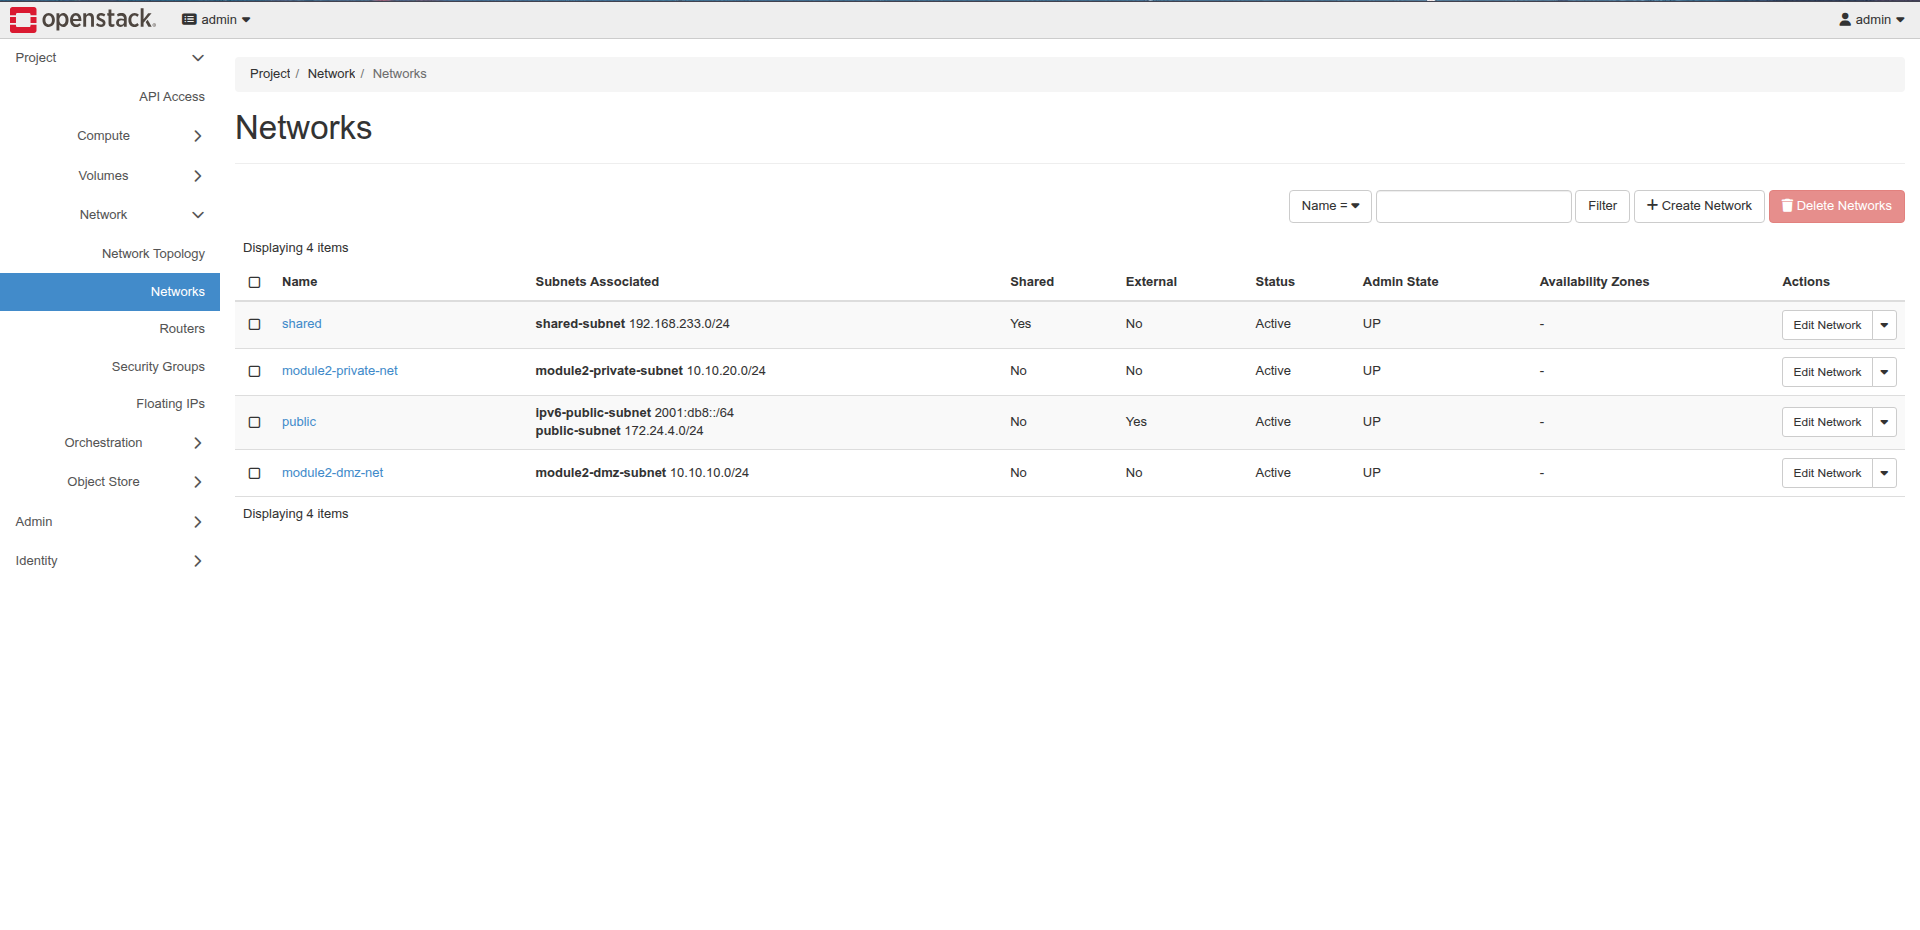
\includegraphics[width=0.88\linewidth]{img/m2-network-list.png}
\caption{Danh sách mạng Neutron hiển thị hai subnet DMZ và Private vừa tạo.}
\label{fig:m2_networks}
\end{figure}

\begin{itemize}
    \item \textbf{Trạng thái các Subnet (Hình~\ref{fig:m2_networks}):} Cả hai subnet tenant (\nolinkurl{10.10.10.0/24} và \nolinkurl{10.10.20.0/24}) đều đã khởi tạo thành công và ở trạng thái sẵn sàng hoạt động.
    \item \textbf{Cổng External Gateway của Router (Hình~\ref{fig:m2_router_overview}):} Nhóm xác nhận bộ định tuyến \texttt{module2-router} đã nhận địa chỉ IP ngoại vi thuộc mạng \texttt{public}, sẵn sàng làm cầu nối ra bên ngoài.
    \item \textbf{Cổng Giao diện Nội bộ (Hình~\ref{fig:m2_router_interfaces}):} Xác nhận \texttt{module2-router} đã liên kết thành công 2 cổng nội bộ đóng vai trò Default Gateway tương ứng cho DMZ (\texttt{10.10.10.1}) và Private (\texttt{10.10.20.1}).
\end{itemize}

\begin{figure}[H]
\centering
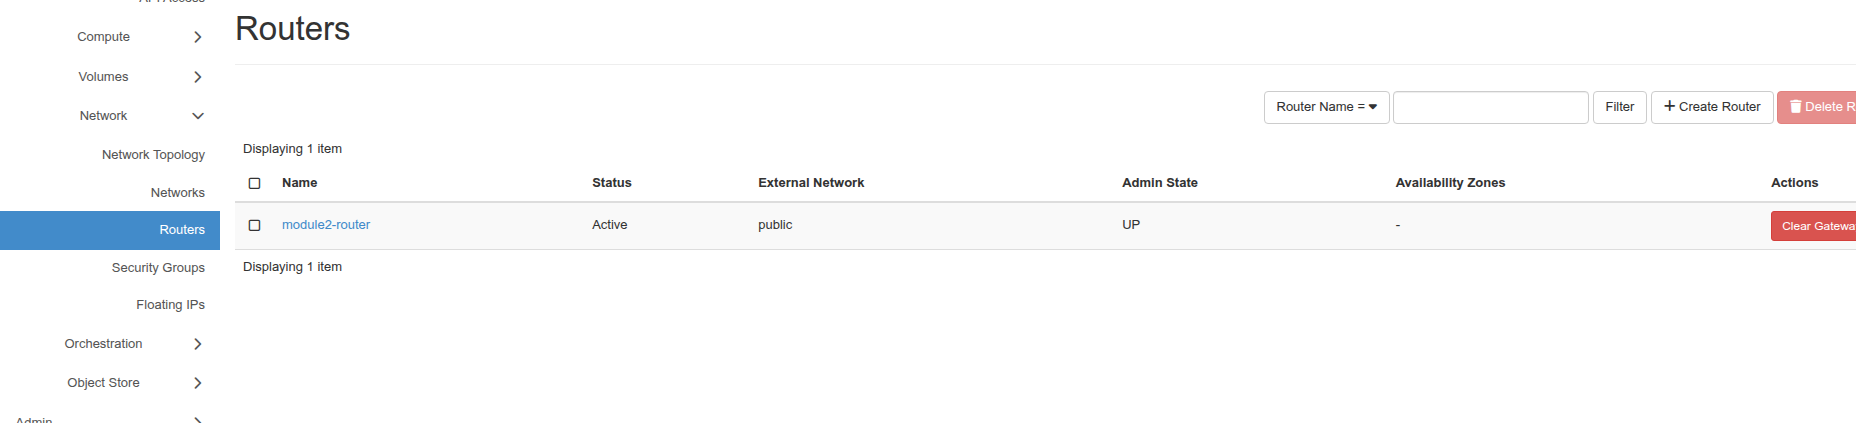
\includegraphics[width=0.88\linewidth]{img/m2-router-external-gateway.png}
\caption{Bộ định tuyến \texttt{module2-router} kết nối uplink ra mạng \texttt{public}.}
\label{fig:m2_router_overview}
\end{figure}

\begin{figure}[H]
\centering
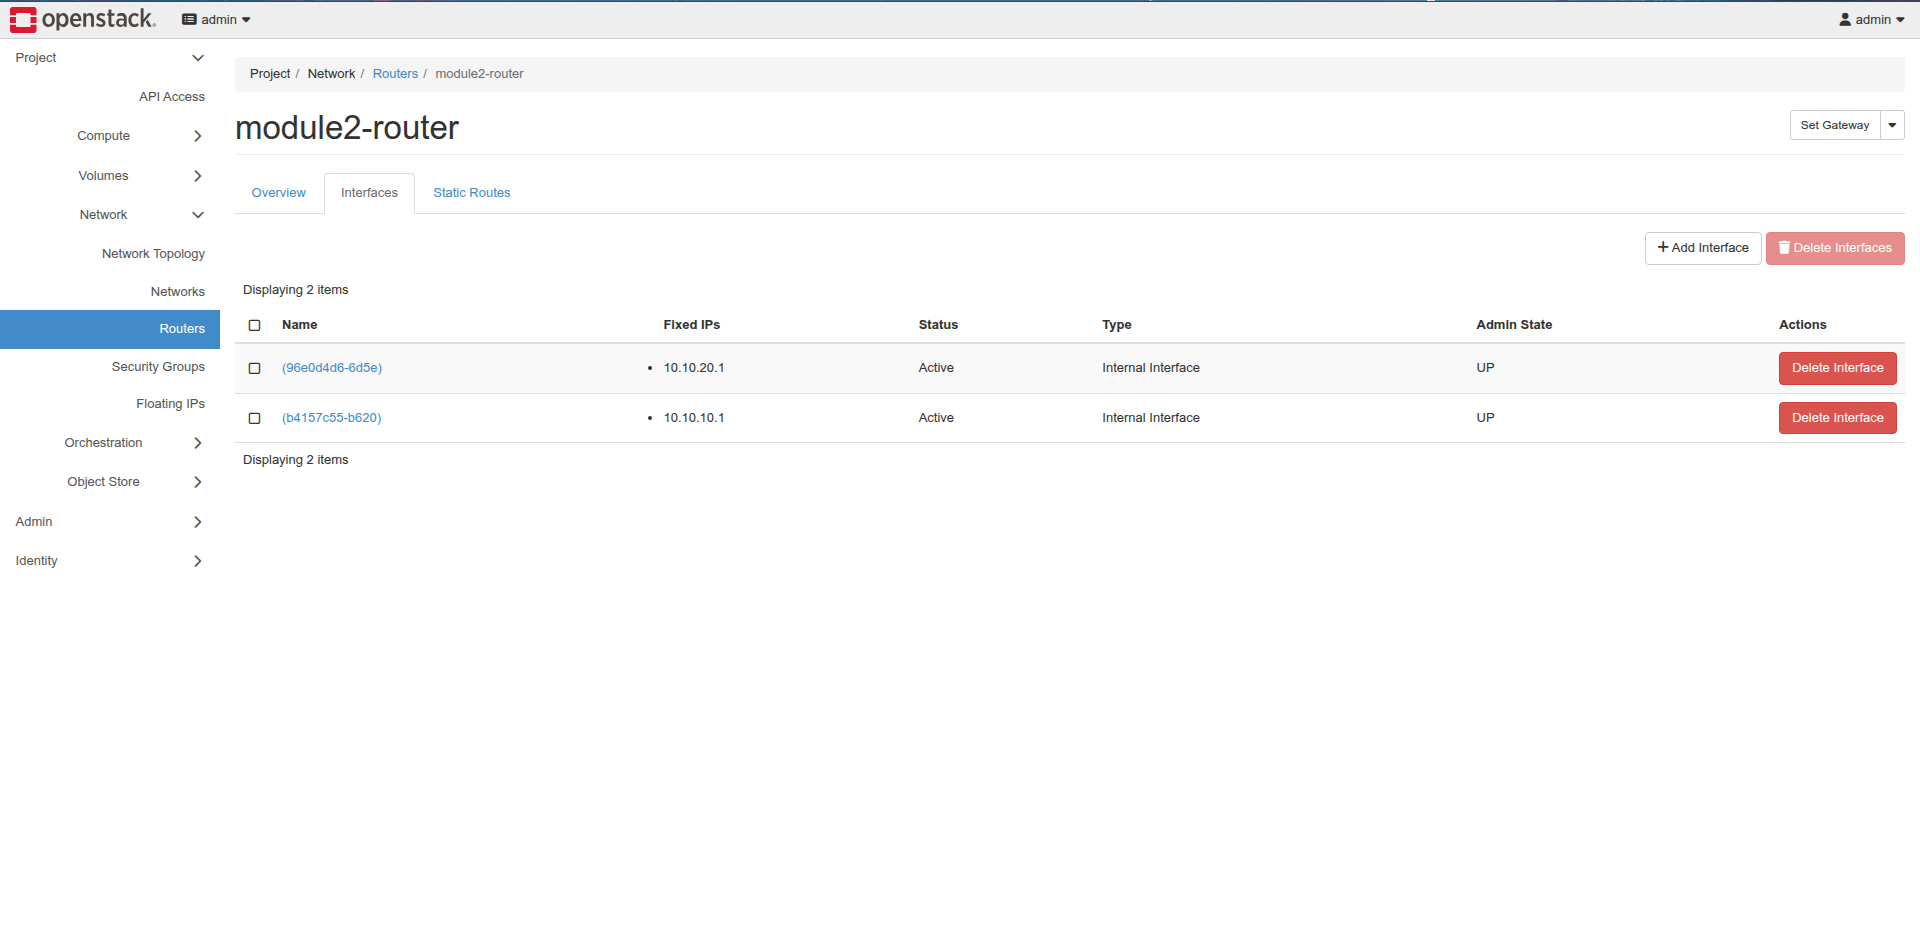
\includegraphics[width=0.88\linewidth]{img/m2-router-internal-interfaces.png}
\caption{Hai cổng giao diện nội bộ (\texttt{10.10.10.1} và \texttt{10.10.20.1}) gắn vào \texttt{module2-router}.}
\label{fig:m2_router_interfaces}
\end{figure}

\begin{itemize}
    \item \textbf{Bảng Phân bổ Cổng Mạng (Hình~\ref{fig:m2_ports}):} Danh sách cổng ảo trong Neutron phản ánh đầy đủ các thành phần hạ tầng, bao gồm cổng dành cho DHCP Agent phục vụ cấp phát IP tự động và các cổng Gateway của router.
    \item \textbf{Sơ đồ Tô-pô Trực quan (Hình~\ref{fig:m2_topology_diagram}):} Sơ đồ tương tác trên bảng điều khiển Horizon minh họa rõ nét cấu trúc phân tầng đa lớp: luồng lưu lượng từ mạng \texttt{public} đi qua \texttt{m2-router} và rẽ nhánh an toàn vào phân vùng DMZ (đường viền đỏ) cùng phân vùng Private (đường viền xanh lá).
\end{itemize}

\begin{figure}[H]
\centering
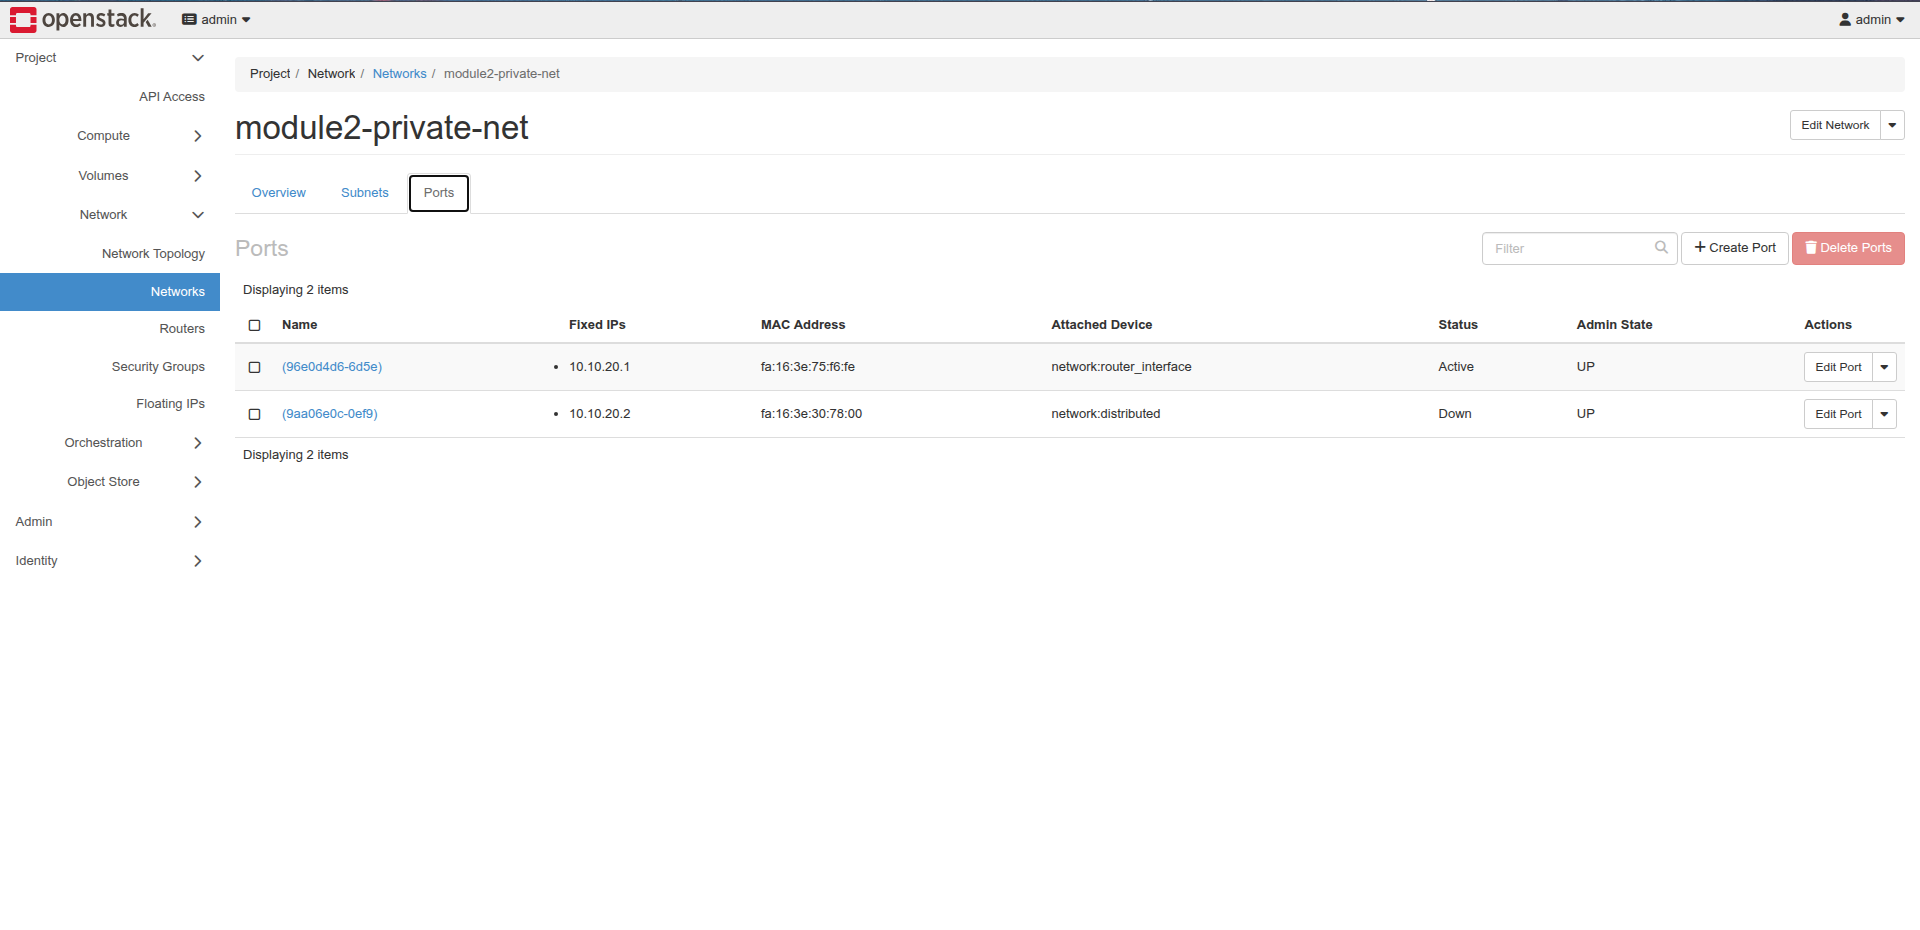
\includegraphics[width=0.88\linewidth]{img/m2-ports-list.png}
\caption{Danh sách cổng mạng trên \texttt{m2-private-net} gồm router gateway và DHCP agent.}
\label{fig:m2_ports}
\end{figure}

\begin{figure}[H]
\centering
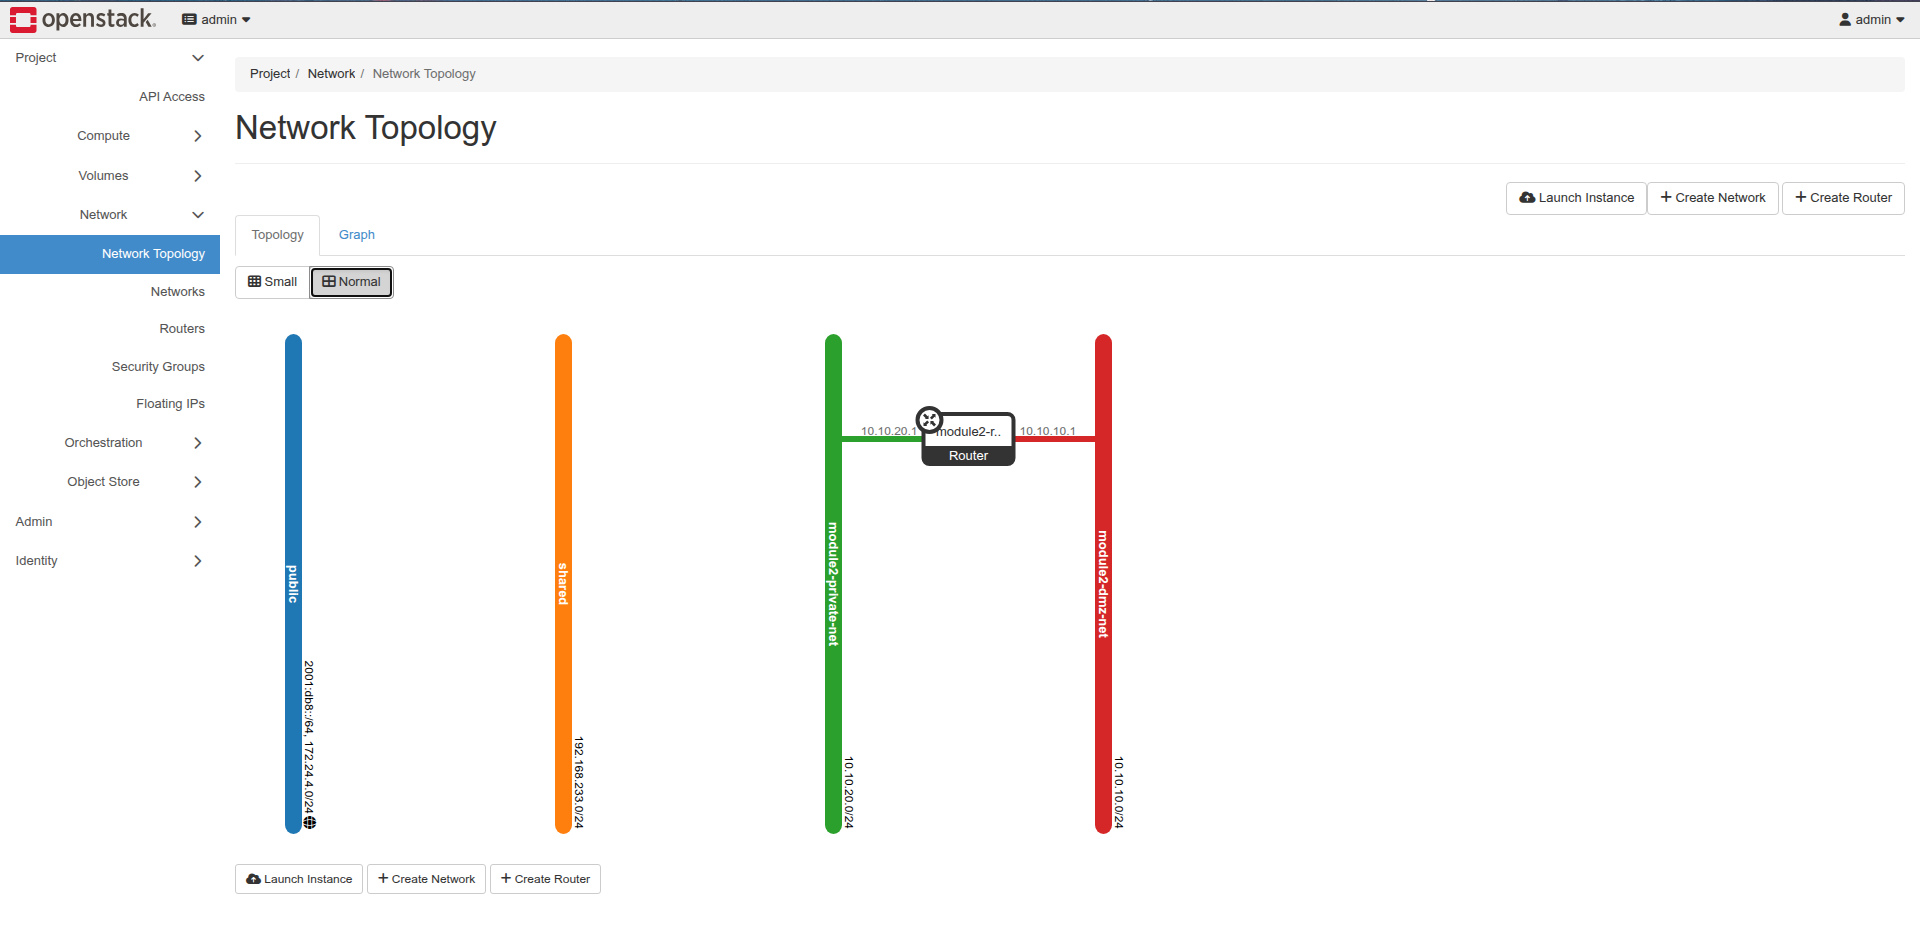
\includegraphics[width=0.88\linewidth]{img/m2-network-topology-diagram.png}
\caption{Sơ đồ tô-pô mạng trực quan trên Horizon thể hiện kiến trúc định tuyến L3.}
\label{fig:m2_topology_diagram}
\end{figure}
